% !TEX root = tesis.tex

\chapter{Related Work}
\label{chap:related_work}


This thesis adds new data and experiments to the fast-growing area of \emph{Mobile Phone Social Network Analysis}.

Earlier works in the general area of \emph{Social Network Analysis} and \emph{Socioeconomic Indices} and their relation to demographic features were drawn from sparse sociological studies~\cite{katz_economics_2001} and nationwide surveys~\cite{deaton1997}. However, the advent of massive clusters of real-world data along with computers big enough to process it completely changed the landscape of human data analysis, both for industry purposes and for academia.

This chapter will discuss several scientific papers in this area which were relevant for the research done in this one.

\section{Correlations of Consumption Patterns in Social-Economic Networks}
\label{sec:leo_correlations}

\cite{leo16correlations} presents correlations between purchasing patterns and socioeconomic position of users from a dataset similar to the one used in this thesis. In particular, the authors have access to a database of credit card purchases for a set of users, with information about the amount of money spent and the general category (MCC) to which the purchase belongs, and also to a cellphone communications graph which allows them to infer the relationship between any two people.

The first of two interesting studies this paper makes is to categorize the population depending on their total spending, and find out the spending level of each user category on one of several aggregated purchase groups. It makes it easy to see the difference in spending for lower income and higher income people: the former group tends to spend comparatively more money in entertainment and retail stores, while the latter group spends more money in hotels and vehicles.

The second study presented in this paper relates to the correlation between people who buy from each of these groups to find categories which are commonly purchased together. Some groups, like \emph{Transportation}, \emph{IT}, or \emph{Personal Services} play a central role and are connected to many other communities, while some others like \emph{Car Sales and Maintenance} and \emph{Hardware Stores} and pairwise connected.

Both of these correlations can be seen intuitively in \cref{fig:paper_yannick}.

\begin{figure}
\centering
\begin{subfigure}[t]{.45\textwidth}
\includegraphicsmaybe{figures/yannick/service_socioeconomic.png}
\label{fig:service_socioeconomic}
\end{subfigure}
\begin{subfigure}[t]{.45\textwidth}
\includegraphicsmaybe{figures/yannick/service_service.png}
\label{fig:service_service}
\end{subfigure}
\caption{Data from the study of categories of purchases. The heatmap on the left side contains the relative purchasing quantities of each category for every socioeconomic level (where 1 is lower and 9 is higher), while the graph on the right side contains the purchase groups which reveals several clusters.}
\label{fig:paper_yannick}
\end{figure}

\section{Inferring Personal Economic Status from Social Network Location}

\cite{Luo2017inferring} shows that an individual's location is highly correlated with its socioeconomic status.
In addition, the paper also finds the interesting observation that some social network patterns mimic the economic inequality patterns, and that there is a significant ($R^2 = 0.96$) correlation between the link diversity of individuals and their financial status.

The results were validated by performing a social marketing campaign for the acquisition of new credit card clients by sending message for individuals that were predicted to be affluent.
Compared to a control group, the users with the most covariance between their links (that is, with the highest link diversity) would more probably request the offered product, which was ideal for affluent users. These results can be seen in \cref{fig:luo2017results}.

\begin{figure}
\centering
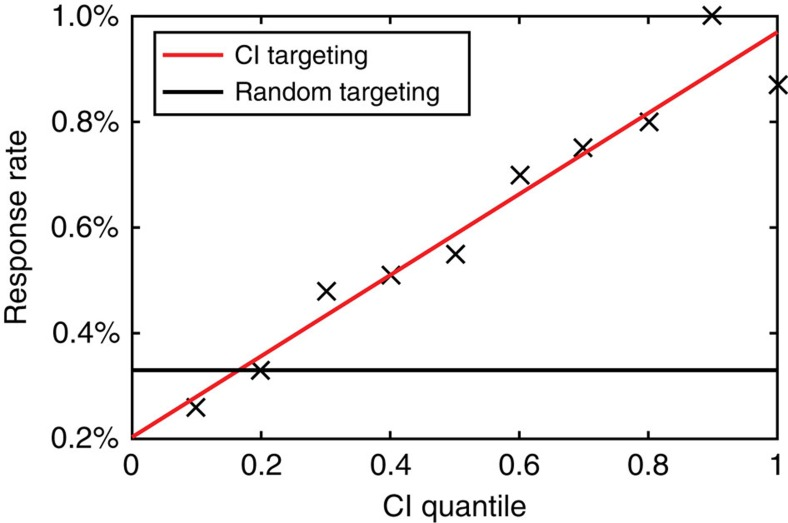
\includegraphics[height=.25\textheight]{figures/luo2017results.png}
\caption{Response rate versus \emph{Collective Influence}, a measure of the variance between links.}
\label{fig:luo2017results}
\end{figure}

Additionally, to prove that the results were not dependent on the validation campaign, the authors produced an \emph{Analysis of Covariance}\cite{wildt1978analysis} on all the features they had access to to test the variance caused by network metrics and other factors.
This resulted in the conclusion that the correlation between collective influence is positive and significant in all groups of geographical communities, across genders, and among all age groups older than 24 years.
Such robust network effects imply that network metrics are a potential indicator for financial status.

Unlike this thesis, this paper is completely observational and doesn't provide a direct inference method for socioeconomic status. However, both its strict methodology and its prediction of \emph{Collective Influence} were useful for completing many parts of this work, specially since the dataset used by Luo et.\ al has many similarities with the one used in this paper.


\section{Socioeconomic Status and Mobile Phone Use}

\cite{blumenstock2010mobile} combines data from direct demographic surveys with \emph{Call Details Records} obtained from a phone company to get demographical data about cellphone users in Rwanda.

The paper combines data about the overall demographic composition of Rwanda with the demographic composition of a representative sample of mobile phone users, along with voluntary survey results and the call history of the survey residents.

Two interesting tests made to measure the socioeconomic status of the respondents, which is particularly hard in a country where a significant percentage most people's income derives from informal channels.

\begin{itemize}
	\item Asking the respondents directly some of the demographic questions previously used in a nation-wide survey from the Rwandan government. This resulted a stark difference in socioeconomic level between the general population and the cellphone-owning people in the survey.
	\item Using this same government survey to compute total expenditures by aggregating expenditures across some subcategories as explained in~\cite{deaton2002}, and then fit the model to the data.
\end{itemize}

With this data it was possible to characterize economic stratification and inequality within the population of mobile phone users. Additionally, using the CDRs, it was possible to characterize graph properties for rich and poor users, in addition to other demographic indicators such as gender. In particular, while the mobile phone population is in general wealthier than the general population of Rwanda, there's still considerable inequality within the group of mobile phone users.

\section{Understanding Individual Human Mobility Patterns}

\cite{gonzalez2008understanding} explores the statistical properties of a population's mobility patterns by using a mobile phone dataset similar to the one used in this thesis. In it, the author finds that the distribution of displacements of users over time can be approximated by a truncated Lévy flight\cite{mandelbrot1982fractal}.

\begin{equation}
	P \left( \Delta r \right) = \left( \Delta r + \Delta r_0 \right) ^{-\beta} \exp \left( -\Delta r / \kappa \right)
\end{equation}

Where $\beta = 1.75 \pm 0.15$, $\Delta r_0 = 1.5 \kilo\meter$, and cutoff values $\kappa | _{D_1} = 400 \kilo\meter$ and $\kappa | _{D_2} = 80 \kilo\meter$.

The author also proposes 3 distinct hypothesis for this behaviour: \encircle{A} each individual follows a Lévy trajectory, \encircle{B} the distribution captures heterogeneity between individuals' movement patterns, or \encircle{C} some heterogeneity coexists with Lévy patterns.

To distinguish between these hypotheses, the author approximated the \emph{Radius of Gyration} $r_g$ for each user, interpreted as the characteristic distance travelled by some user at some time. While the ensemble of Lévy agents had a significant level of heterogeneity, the author suggests that this is because of the big range of mobility patterns in individuals, thus ruling out hypothesis \encircle{A}.

Conversely, the data also shows that users with small $r_g$ travel mostly over small distances, whereas those with large radius display a combination of small and large jump sizes. After rescaling all the distributions with this value, the author shows that the data collapsed into a single curve.
Therefore, travel patterns of individual user may be approximated by a Lévy flight up to a distance characterized by $r_g$; with this definition we can see that large displacements are statistically absent.
This indicates that the jump size distribution of $P \left( \Delta r \right)$ is the convolution between the statistics of individual trajectories $P \left( \Delta r_g \mid| r_g \right)$ and the population heterogeneity $P \left( r_g \right)$, which is consistent with hypothesis \encircle{C}.

This study demonstrates that the individual trajectories are characterized by the same $r_g$-independent  probability distribution, and this suggests that the statistical elements of individual categories are indistinguishable after rescaling. Therefore, this has the basic ingredients of realistic agent-based models. Given the known correlations between spatial proximity and social links, this could help quantify the role of space in network development and evolution, and improve the general understanding of diffusion processes.

\section{Link-based Classification}

\cite{lu2003link} proposes a statistical framework for modeling distributions between linked documents (such as relational databases or URLs in websites) to use in machine learning. This is a hard problem, since naïvely applying traditional statistical inference procedures, that assume that links are independent, can lead to inappropriate conclusions\cite{jensen1999statistical}.

The study proposes using several features for these links, while later using a logistic regression model for each of the features. Since the original problem required multilabeling classification, the study calculates the probability of each label given the features in a one-against-others model and picked the one for the highest posterior probability.

The authors also propose an iterative algorithm to compute the category of each link depending on the labels of their neighbour (which change on each step), which reports an improvement in classification accuracy.

\section{Socioeconomic Correlations in Communications Networks}

\cite{leo2015socioeconomic} uses a similar dataset to the one used in this thesis that collects communication and bank information about individuals, and shows that consumption patterns are correlated with identified socioeconomic classes leading to social stratification in a similar way to the paper discussed in \ref{leo_correlations}.
In addition, the paper introduces a correlation between merchant categories.

Given the set of users' purchases, the authors separate it into 17 categories, and measure the fractional distribution of spending for each one as the amount of money each user spent into each category over the total money spent.
As expected, people in lower socioeconomic classes spend more in groups associated with essential needs, such as retail stores, gas stations, or service providers, while people in higher socioeconomic classes spend the majority of the money on jewelry, automobiles, and professional services.

\section{A Comparative Study of Social Network Classifiers}

In \cite{oskarsdottir2016}, the authors present several methods to address machine learning classification in social networks and other graph-related structures.
The methods are separated into several categories.

\begin{enumerate}
	\item \emph{Relational Classifiers}, which infer labels for each node based on the strength of the links to other nodes and the labels to those nodes.
	\item \emph{Collective Inference} methods, which infer labels for the nodes of the network while taking into account how the inferred labels affect each other.
\end{enumerate}

The paper uses telco data from many separate sources for testing, and uses a single logistic regression model to predict the correct label from the given features.
Despite testing it with several metrics, there are some feature generating methods that are better than the other ones in every single one.

The way this paper presented several features, and the methods it used for testing, were a great inspiration for the work in this thesis.
